% --------------------------------------------------------------
% This is all preamble stuff that you don't have to worry about.
% Head down to where it says "Start here"
% --------------------------------------------------------------
\documentclass[12pt]{article}

\usepackage[margin=1in]{geometry}
\usepackage{amsmath,amsthm,amssymb}
\usepackage{graphicx,ctable,booktabs}

% ----------------------------------------------------------------------------------------------------------------------------------------------
% Commands
%-----------------------------------------------------------------------------------------------------------------------------------------------
\newcommand{\justif}[2]{&{#1}&\text{#2}}
\newcommand{\N}{\mathbb{N}}
\newcommand{\Z}{\mathbb{Z}}
\newcommand{\R}{\mathbb{R}}


\newenvironment{theorem}[2][Theorem]{\begin{trivlist}
\item[\hskip \labelsep {\bfseries #1}\hskip \labelsep {\bfseries #2.}]}{\end{trivlist}}
\newenvironment{lemma}[2][Lemma]{\begin{trivlist}
\item[\hskip \labelsep {\bfseries #1}\hskip \labelsep {\bfseries #2.}]}{\end{trivlist}}
\newenvironment{exercise}[2][Exercise]{\begin{trivlist}
\item[\hskip \labelsep {\bfseries #1}\hskip \labelsep {\bfseries #2.}]}{\end{trivlist}}
\newenvironment{problem}[2][Problem]{\begin{trivlist}
\item[\hskip \labelsep {\bfseries #1}\hskip \labelsep {\bfseries #2.}]}{\end{trivlist}}
\newenvironment{question}[2][Question]{\begin{trivlist}
\item[\hskip \labelsep {\bfseries #1}\hskip \labelsep {\bfseries #2.}]}{\end{trivlist}}
\newenvironment{corollary}[2][Corollary]{\begin{trivlist}
\item[\hskip \labelsep {\bfseries #1}\hskip \labelsep {\bfseries #2.}]}{\end{trivlist}}
\newenvironment{definition}[2][Definition]{\begin{trivlist}
\item[\hskip \labelsep {\bfseries #1}\hskip \labelsep {\bfseries #2.}]}{\end{trivlist}}
\newenvironment{remark}[2][Remark]{\begin{trivlist}
\item[\hskip \labelsep {\bfseries #1}\hskip \labelsep {\bfseries #2.}]}{\end{trivlist}}
\newenvironment{alt_def}[2][Alternative Definition]{\begin{trivlist}
\item[\hskip \labelsep {\bfseries #1}\hskip \labelsep {\bfseries #2.}]}{\end{trivlist}}
\newenvironment{example}[2][Example]{\begin{trivlist}
\item[\hskip \labelsep {\bfseries #1}\hskip \labelsep {\bfseries #2.}]}{\end{trivlist}}
\newenvironment{prop}[2][Proposition]{\begin{trivlist}

\item[\hskip \labelsep {\bfseries #1}\hskip \labelsep {\bfseries #2.}]}{\end{trivlist}}

\begin{document}
% --------------------------------------------------------------
% Start here
% --------------------------------------------------------------
\title{CMPSC 448: Informative Tweets and Retweets}
\author{Scott Bickel, Brian Golden, Steven Styer}
\date{\today}
\maketitle
\tableofcontents
\section{Introduction}
The online social network Twitter, allows users to post 140 character long messages called {\it tweets} which can be seen by other Twitter users. In the past few years, Twitter has become increasingly popular and is a powerful medium for influence and awareness. Thus,  determining the informative value of a tweet and determining whether a tweet will be retweeted, is of great importance and has numerous applications. For our project we focused on both of these questions and took a supervised learning approach.\\
\indent
In determining the informative value of a tweet, we restricted the problem to classification, i.e. can we determine whether or not a tweet is informative? We were able to achieve an accuracy of 87.5\% using a Support Vector Machine. Furthermore, we quantitatively determined which explanatory variables (features) were contributing the most to the response variable (target) using logistic regression.\\
\indent
 In determining whether a tweet will be retweeted, we were able to achieve 72\% accuracy, using a classifying decision tree. As a further test of curiosity to see how ensemble methods perform, we ran a Random Forest algorithm on the data and further improved our accuracy to 78\%. The remainder of this report provides full details of our data, features, models, evaluations and conclusions.
\section{Datasets}
Throughout our experimentation and analysis, we used two datasets of sizes 600,000 and 2,000,000 million tweets. The tweets were collected over timespans of 5-12 weeks matching a small subset of about 10 {\it hashtags}. A hashtag is a word in a tweet prefixed with the '\#' symbol, and is used to tag a tweet. An {\it ngram} is n words contiguous in a sentence. We extracted all 1grams, 2grams, and 3grams for all tweets. Furthermore, we compute the frequency of each ngram. Each of the datasets has the following attributes:
\begin{enumerate}
	\item \textbf{Tweet ID} -- a unique identifier for the tweet
	\item \textbf{Source User ID} -- the ID of the user that posted the tweet
	\item \textbf{Retweet User ID} -- the user that posted the original tweet being retweeted or -1 if the tweet is not a retweet
	\item \textbf{Website} -- the address of the website in the tweet if it exists
	\item \textbf{Tweet Time} -- the time in which the tweet was posted
	\item \textbf{Hash Tag} -- the hashtag of that tweet that was matched to find the tweet
\end{enumerate}
For determining whether or not a tweet is informative, we decided to use a supervised learning algorithm. Hence, we had to manually label a random sample of 1000 tweets from our dataset to obtain the classification. This manual labelling was done by a third party in order to maintain consistency and eliminate any of our own bias.
\subsection{Quality of Models Classifying Informative Tweets}
From the various methods and metrics mentioned in the above subsections, we can say that the models trained with these features are of decent quality. Again, assuming our baseline prediction is approximately 50\% (i.e. by guessing you have about a 50/50 chance of correctly classifying a tweet) than a support vector machine scored at 87\% accuracy is a good improvement over that. However, there is certainly more work to be done on feature refinement, since one feature in each feature vector is weighted much higher than the others. \\
\\
It is worth noting that models trained to classify tweets as informative or not should have training and testing sets of tweets that have been identified as being from relatively similar topics. This is to ensure that using n-grams as features makes sense, e.g. tweets about the latest congressional elections should not be classified by a model trained on tweets about the NFL draft. 
\section{Informative Tweets}
For our purposes, we will call an {\it informative tweet} a tweet which, by nature of its existence, has purpose and value transferring information to other users and people. It is worth noting that this is a relatively imprecise definition, but that without explaining what we consider to be an informative tweet, our classification will be meaningless. All tweets that are not informative are simply designated as a {\it non-informative tweet}, or rather a tweet which may provide entertainment, make non-factual commentary, or hold a conversation with one or more Twitter users. 
\\
\\
Determining if a tweet is informative or not is a binary classification. As such, we chose to use support vector machines to classify tweets into one of two categories. 
\subsection{Results}
Initially we did not achieve much success. In fact, we decided to start over after Milestone 2 because we had some misunderstandings with some key concepts. We restarted with the following features for initial experimentation:
\begin{enumerate}
	\item \textbf{reply} -- whether or not the tweet is a reply
	\item \textbf{retweet} -- whether or not the tweet is a retweet
	\item \textbf{retweet count} -- the number of retweets of the tweet.
\end{enumerate}
We believed that these simple features could be a basic starting point for our investigation. With a 5-fold cross validation, we achieved an average accuracy score of $0.567$. As our informative and non-informative classes are roughly equal in size, this classification would not be much better than always guessing. The following figure shows a confusion matrix visualization:
\begin{figure}[h]
\centering
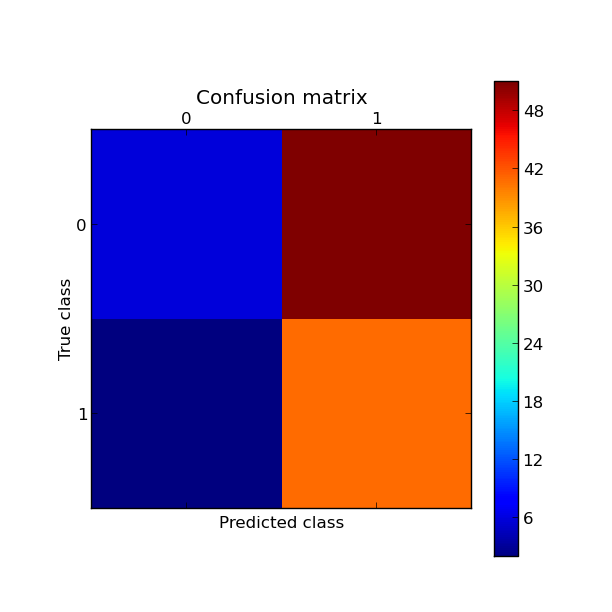
\includegraphics[width=14cm]{init_cfnmat.png}
\caption{Initial Confusion Matrix where 0 is the non-informative class and 1 is the informative class}
\label{fig:cfm}
\end{figure}\\
We found the visualization of the confusion matrix to be extremely helpful. From the plot we could see that we over-predicted the informative class when the true class was non-informative. Looking at our features, we saw how this could happen. Specifically, the only feature that potentially gives us non-informative information is the reply feature. Hence, we decided to add more features.
\subsection{Feature Refinement}
We believed that we did not have enough features so we intuitively thought about what would make a tweet informative or non-informative. We thought about various other factors such as: user importance, named entities, links to additional information, and hashtags. User importance is can be determined by using centrality measures in a graph. We accomplished this with the python library {\it networkx} and used the eigenvector centrality algorithm. For named entities, we discovered the {\it Stanford NER} classifier. The classifier gave us people, organizations and locations mentioned inside tweets and so we converted them into counts. For links to additional information, we noticed that a lot of Twitter users that were trying to spread their influence would include additional information in their Tweet as a link. Lastly, we decided not to use hashtags/topics in our classification as we realized how much larger our features would become.
\subsection{Evaluation}
Now our new feature list includes the following:
\begin{enumerate}
	\item \textbf{reply}                    -- the tweet is a reply to another user 
	\item \textbf{retweet}                  -- the tweet is a retweet of another user 
	\item \textbf{retweet count}            -- the number of retweets the tweet has  
	\item \textbf{eigenvector centrality}   -- the user importance of the user who sent the tweet 
	\item \textbf{number of people}         -- the number of people mentioned in the tweet
	\item \textbf{number of organizations}  -- the number of organizations mentioned in the tweet
	\item \textbf{number of locations}      -- the number of locations mentioned in the tweet
	\item \textbf{website}                  -- the website linked to in the tweet
\end{enumerate}
Again, we performed a 5-fold cross validation but this time attained a mean score of $87.5$\%! Of course we attributed this to the additional features we added. Later we will more closely investigate which features were responsible for our much improved accuracy by attempting to measure which feature gave us the most information. Right now, we will show our evaluation of these results through metrics and visualizations.
\\
\\
Again we made a confusion matrix of our new results:
\begin{figure}[h]
\centering
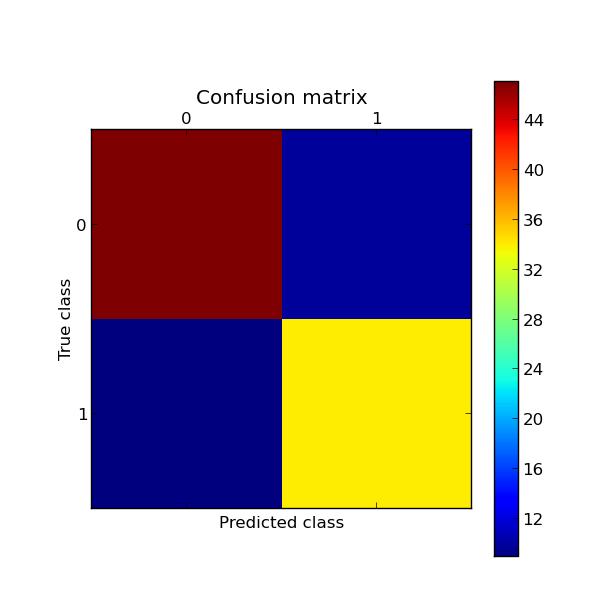
\includegraphics[width=14cm]{improved_cfm1.png}
\caption{Final Confusion Matrix where 0 is the non-informative class and 1 is the informative class}
\label{fig:cfm2}
\end{figure}\\
\\
\\
The following are the metrics for the confusion matrix: \\
\\
\begin{centering}
\begin{tabular}[b]{l||c} \\
    \textbf{Metric} &\textbf{Value} \\
    \hline 
    \hline
    \textbf{accuracy} &0.8650 \\
    \hline
    \textbf{precision} &0.8611 \\
    \hline
    \textbf{true positive rate} &0.8857 \\
    \hline
    \textbf{false positive rate} &0.1579 \\
    \hline
    \textbf{true negative rate} &0.8421 \\
\end{tabular}
\end{centering}
\\
\\
From the confusion matrix we can see that we greatly improved our accuracy in predicting the $0$-class i.e. the non-informative tweets. In fact, our accuracy in predicting non-informative tweets is about as good as it can be. In contrast, the confusion matrix clearly shows that there is room for improvement with the informative class. 
\\
\\
An additionally useful illustration of the classifier's performance is a receiver operating characteristic (ROC) curve. Such plots allow us to see how good the model is at minimizing the false positive rate while maximizing the true positive rate of classifying tweets; this is essentially a cost/benefit analysis of how to vary the parameters of the model to make the best classifications in the future. As such, the best model would be the one with the largest area under the curve, i.e. the integral of the plot (often referred to as simply the AUC or ROCAUC). The following is a plot of the ROC curve for our classifier: \\
\\
\begin{figure}[h]
\centering
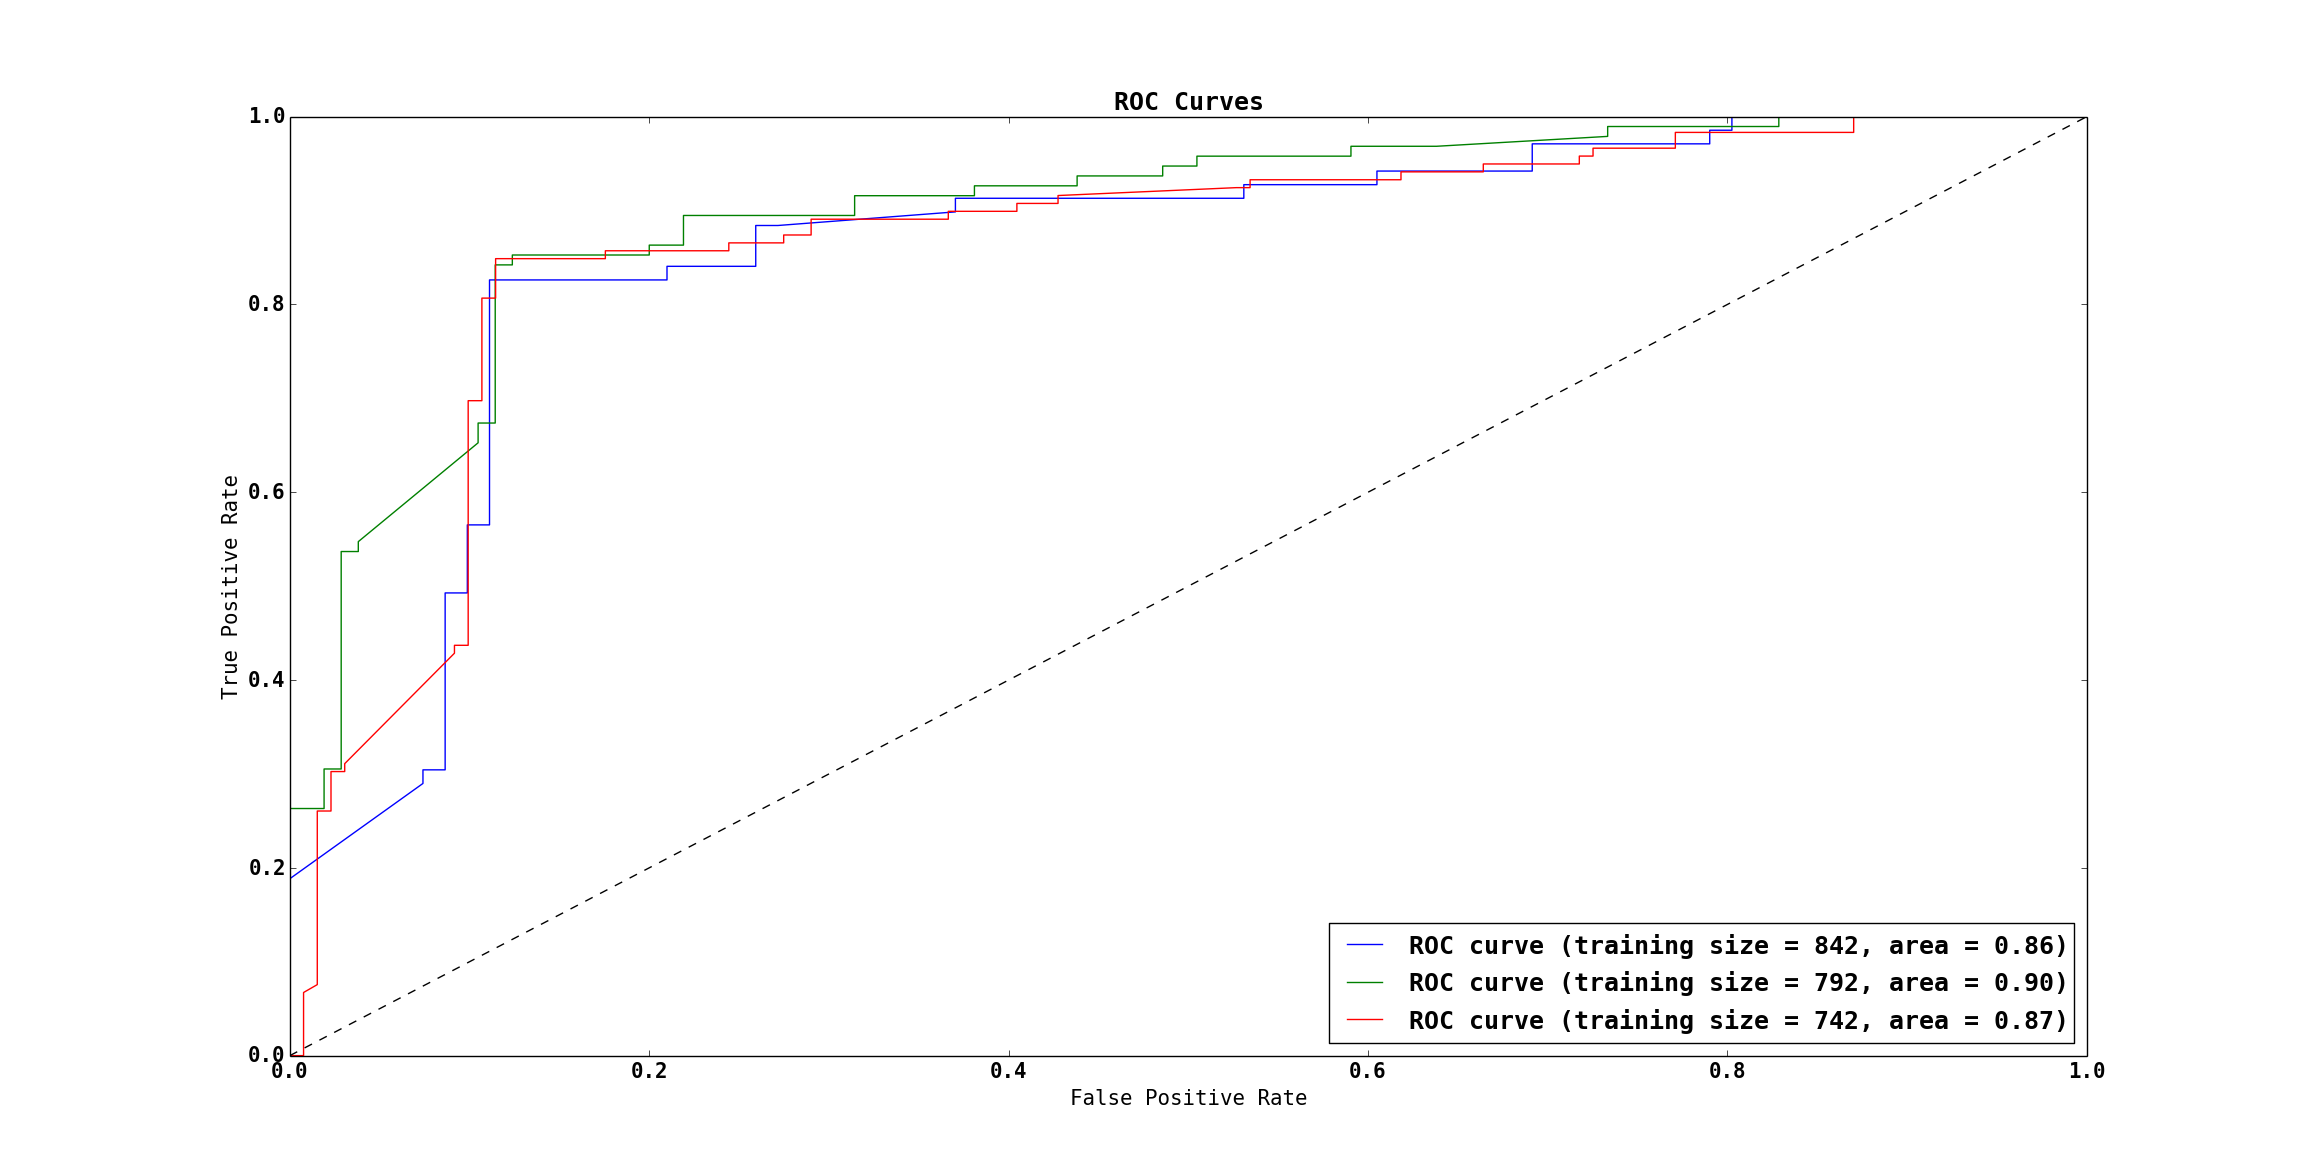
\includegraphics[width=16cm]{final_roc.png}
\caption{Final ROC Curve with three test runs}
\label{fig:roc}
\end{figure}\\
\\
\\
This ROC curve shows that our model is most effective when using a test set size of 250 data points, or a training set size of 792 data points. This trained model had a ROCAUC of 0.90, which is a considered to be an excellent test; a good model is one where 
\[0.8 \le ROCAUC \le 0.9\] 
and an excellent model is one where 
\[0.9 \le ROCAUC \le 1.0\] 
So the model trained on 792 data points is considered to be an excellent test, bordering below on a good test. \cite{rocarea}
From this we can say that models trained to make future predictions on the informativeness of tweets should be trained with approximately 792 data points to maximize the ROCAUC of the model and therefore make the least costly classifications. 
\subsection{Logistic Regression}
As mentioned earlier, we will now dig into our features, (explanatory variables) and determine which one contributes the most to our response variable (target). We can do this via the coefficients found after fitting a regression model. As our response variable is categorical, we used a logistic regression model. Specifically, we used the R programming language for fitting the model. The following table shows the logistic regression coefficients:\\
\\
\begin{centering}
\begin{tabular}[b]{l||c|c|c|c|}
         \textbf{} &\textbf{Estimate} &\textbf{Std. Error} &\textbf{$z$ value} &\textbf{Pr($>|z|$)} \\
         \hline    
         \hline
         \textbf{intercept} &-2.9502986 &0.2514704 &-11.732 & 2e-16 \\
         \hline
         \textbf{website} &4.2864985 &0.2340763 &18.312 & 2e-16 \\
         \hline
         \textbf{retweet} &-0.7862853 &0.4776865 &-1.646 &0.099758 \\
         \hline
         \textbf{reply} &1.1823990 &0.2356566 &5.017 &5.24e-07 \\
         \hline
         \textbf{retweet count} &-0.0007451 &0.0004794 &-1.554 &0.120103 \\
         \hline
         \textbf{number of people} &0.0610550 &0.1821874 &0.335 &0.737533 \\
         \hline
         \textbf{number of organizations} &0.7080103 &0.1863903 &3.799 &0.000146 \\
         \hline
         \textbf{number of locations} &0.5265293 &0.1910123 &2.757 &0.005842 \\
         \hline
         \textbf{eigenvector centrality} &-8.6687808 &6.6922327 &-1.295 &0.195200 \\
       \end{tabular}
       \end{centering}\\
\subsection{Evaluation}
To evaluate this model we compute a p-value of the hypothesis: ``Can we do better than the Null model''. R gave us a p-value of $1.036467e-143$, clearly the logistic regression model is statistically significant. This can be further corroborated by the fact that a 5-fold cross validation achieved a mean score of 87.4\%.\\
\indent We note that this logistic regression model does not classify any more accurately than the classifying support vector machine. However, with the logistic regression model we were able to uncover more about our features. Specifically, from the above table we can conclude that features: {\it website}, {\it reply}, and {\it number of organizations} are statistically significant with level $0.001$. The features: {\it number of locations} and {\it retweet} are statistically significant with levels $0.01$ and $0.1$ respectively. The remaining features were not statistically significant. 
\subsection{Indicative Features}
To determine which features contribute the most to the response variable we can look at the coefficients. In logistic regression this is can be done by finding the odds ratio. We can find an odds-ratio increase for every unit increase in a coefficient as follows: \\
Our logistic equation has the form:
\[
  F(x) = \frac{1}{1+e^{-\beta\cdot x}} \quad\text{where $\cdot$ is the dot product}
\]
$F(x)$ is the probability of success i.e. the probability of a tweet being informative. Solving for $\beta\cdot x$, we get the {\it logit}:
\[
   \ln\left(\frac{F(x)}{1-F(x)}\right) = \beta\cdot x = \beta_o+\beta_1x_1+\ldots+\beta_8x_8
\]
$\frac{F(x)}{1-F(x)}$ is the odds of $x$. Hence, each unit increase of a coefficient, tells us the log-odds increase of the response. We can simply exponentiate $\beta\cdot x$ and get the actual odds. The following shows the odds-ratio for each feature and their corresponding confidence interval:\\
\\
\begin{centering}
  \begin{tabular}[b]{l||c|c|c} 
    \textbf{} &\textbf{OddsRatio} &\textbf{2.5\%} &\textbf{97.5\%} \\
    \hline
    \textbf{Intercept} &$5.232408e-02$ &$3.128652e-02$ &$0.08398853$ \\
    \hline
    \textbf{website} &7.271142e+01 &4.672998e+01 &117.21668674 \\
    \hline
    \textbf{retweet} &4.555338e-01 &1.746192e-01 &1.14087614 \\
    \hline
    \textbf{reply} &3.262191e+00 &2.079795e+00 &5.25279198 \\
    \hline
    \textbf{retweet count} &9.992551e-01 &9.982375e-01 &1.00004548 \\
    \hline
    \textbf{number of people} &1.062957e+00 &7.415222e-01 &1.51527342 \\
    \hline
    \textbf{number of organizations} &2.029948e+00 &1.417157e+00 &2.94361510 \\
    \hline
    \textbf{number of locations} &1.693046e+00 &1.175115e+00 &2.47795383 \\
    \hline
    \textbf{eigenvector centrality} &1.718685e-04 &3.433019e-10 &41.28819208 \\
  \end{tabular}
\end{centering}\\
\\
Hence we can conclude that the website feature is most indicative of whether or not a given tweet is informative. To determine the validity of this result, we propose that a further experiment could be done where the manually labeled targets are crowd-sourced to potentially better reflect what it means for a tweet to be informative.
\section{Predicting Retweets}
To predict whether a tweet would be retweeted, we used a classifying decision tree. Specifically, we used the R programming language to fit the model. We note that this time we did not manually label anything. For our best classification, we ended up using a much larger sample size of 10,000 tweets. Out of further curiosity, we also classified with the Random Forest algorithm which improved our accuracy even further.
\subsection{Results}
Initially we achieved an accuracy of about 59\%, which is quite bad considering the retweeted class has a size of 41\% and we could get this result by simply guessing. In our initial experiment, we used the following 6 features on a dataset of size 1,000:
\begin{enumerate}
	\item \textbf{website}                  -- whether or not there is a website embedded in the tweet
	\item \textbf{reply}                    -- whether or not the tweet is a reply to another user
	\item \textbf{eigenvector centrality}   -- the user importance of the tweet 
	\item \textbf{number of locations}      -- the number of named-entity locations in the tweet
	\item \textbf{number of people}         -- the number of named-entity people in the tweet
	\item \textbf{number of organizations}  -- the number of named-entity organizations in the tweet
\end{enumerate}
\subsection{Feature Refinement}
We again did a logistic regression for some further diagnostics and we consistently saw that the eigenvector-centrality feature was superfluous. The reason for this is probably due to the fact that models are trained using relatively small slices of the data set, as we cannot collect every tweet ever created on Twitter. From our diagnostics we also saw the named-entity features increased our accuracy only marginally and because of their computational requirements, we decided to stop using them as well. Instead, we extracted the top 500 most frequently occurring 1-grams, 2-grams, and 3-grams from the entire dataset. An {\it n-gram} is a sequence of n items, in this case words or terms. These n-grams can essentially be used as an inexpensive method of identifying topics and common terminology discussed in tweets. We used all 500 of these ngrams as binary features, i.e. 1 means that the given ngram is in the text of the tweet and 0 means that it is not in the text of the tweet. With the above considerations, we decided to sample a much larger testing set and decided to randomly sample 10,000 rows. This gave us an initial accuracy of 69\%. With some further refinements, we were able to improve our accuracy by another 3\%.
\newpage
\subsection{Evaluation}
First, we decided to re-include the website and reply features. Next, in order to reduce model complexity and hence decrease generalization error, we searched for the best value of the complexity parameter. This was computed with a cross-validation and the following plot shows the search: \\
\begin{figure}[h]
\centering
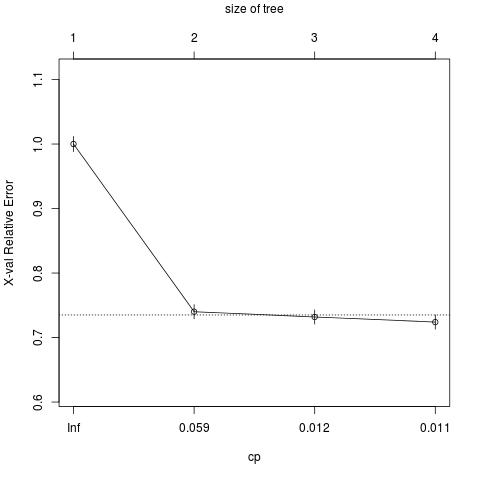
\includegraphics[width=12cm]{plotcp.jpeg}
\caption{Plot showing the best value for the complexity parameter}
\label{fig:dtree}
\end{figure}\\
With the value of our complexity parameter, we passed it to a method to 'prune' the tree. The following shows our less complex, decision tree:
\newpage
\begin{figure}[h]
\centering
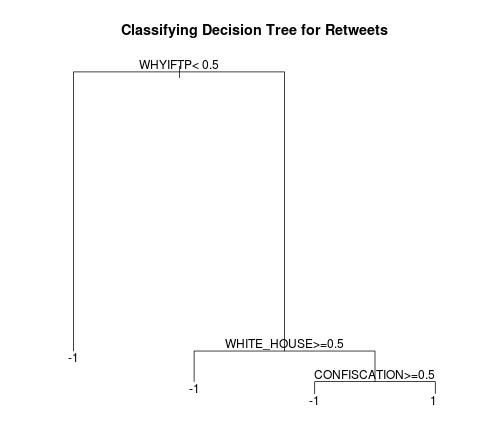
\includegraphics[width=12cm]{dtree.jpeg}
\caption{The classifying decision tree}
\label{fig:cp}
\end{figure}
With these fine tunings, we were able to achieve our claimed accuracy of 72\%. This accuracy is better than just simply guessing the classes because the class sizes are about 58\% to 42\%. However, we were not satisfied with the decision tree and our results, and so we decided to additionally test out the R implementation of the Random Forest algorithm. From discussions in class, we were curious to test the claim that ensemble methods achieve great success. With the Random Forest alone, we immediately saw an increase in model accuracy. The following shows the confusion matrix for this classification:\\
\\
\begin{centering}
\begin{tabular}[b]{l||c|c|c} \\
    \textbf{} &\textbf{-1} &\textbf{1} &\textbf{class error}\\
    \hline 
    \textbf{-1} &4542 &1284 &0.2203913\\
    \hline
    \textbf{1} &994 &3180 &0.2381409 \\
\end{tabular}
\end{centering}
\\
\\
As we can see, we achieved about 6\% more accuracy by simply running a different algorithm! Of course this higher accuracy had the trade-off of running time, but it was certainly feasible. More investigations are definitely necessary to determine whether or not a tweet will be retweeted. One immediate suggestion is that all of our features are of the same type, namely topical. While topics do play a role in classification, other factors in the dynamics of tweets certainly exist and our models do not account for this. For example, network metrics, locations, and tweet times are features that we cam immediately think of.
\section{Conclusion}
Determining whether tweets are informative and whether they will be retweeted are of great importance. We found this project very engaging and we hope with more time that we can further improve our questions, features, and measurements.  Looking back to when we first started this project, we have travelled a great distance -- we knew nothing. We now have much more insight about how to pick a model, how to finely tune that model and how to measure its performance. Furthermore, we saw many machine learning/statistical concepts come to life through this project and we more adequately learned how to apply our knowledge in both theory and practice. In theory, we made sense of our data using concepts such as the bias-variance trade-off, model selection, and cross-validation. In practice, we learned about the importance of feature selection/refinement, and gained more experience processing data using python, MySQL, and R. Furthermore, we learned more valuable lessons with version control using GIT, and how to effectively collaborate as a team. With more time, we hope to uncover the mysteries behind these two questions and improve our capabilities in analyzing problems in the machine learning domain.
\begin{thebibliography}{4}
\bibitem{rocarea}
    Thomas G. Tape, MD,
    \emph{Interpreting Diagnostic Tests}. 
    http://gim.unmc.edu/dxtests
\end{thebibliography}
\end{document}
